\let\negmedspace\undefined
\let\negthickspace\undefined

\documentclass[journal]{IEEEtran}
\usepackage[a5paper, margin=10mm, onecolumn]{geometry}
%\usepackage{lmodern} % Ensure lmodern is loaded for pdflatex
\usepackage{tfrupee} % Include tfrupee package

\setlength{\headheight}{1cm} % Set the height of the header box
\setlength{\headsep}{0mm}     % Set the distance between the header box and the top of the text

\usepackage{gvv-book}
\usepackage{gvv}
\usepackage{cite}
\usepackage{amsmath,amssymb,amsfonts,amsthm}
\usepackage{algorithmic}
\usepackage{graphicx}
\usepackage{textcomp}
\usepackage{xcolor}
\usepackage{txfonts}
\usepackage{listings}
\usepackage{enumitem}
\usepackage{mathtools}
\usepackage{gensymb}
\usepackage{comment}
\usepackage[breaklinks=true]{hyperref}
\usepackage{tkz-euclide} 
\usepackage{listings}
% \usepackage{gvv}                                        
\def\inputGnumericTable{}                                 
\usepackage[latin1]{inputenc}                                
\usepackage{color}                                            
\usepackage{array}                                            
\usepackage{longtable}                                       
\usepackage{calc}                                             
\usepackage{multirow}                                         
\usepackage{hhline}                                           
\usepackage{ifthen}                                           
\usepackage{lscape}
\begin{document}

\bibliographystyle{IEEEtran}
\vspace{3cm}

\title{2.10.39}
\author{EE25BTECH11010 - Arsh Dhoke}
{\let\newpage\relax\maketitle}

\renewcommand{\thefigure}{\theenumi}
\renewcommand{\thetable}{\theenumi}
\setlength{\intextsep}{10pt}
\numberwithin{equation}{enumi}
\numberwithin{figure}{enumi}
\renewcommand{\thetable}{\theenumi}

\parindent 0px
\textbf{Question:} \\
Let $\vec{a}=2\vec{i}+\vec{j}+\vec{k}$,\quad
$\vec{b}=\vec{i}+2\vec{j}-\vec{k}$ and a unit vector $\vec{c}$ be coplanar.
 If $\vec{c}$ is perpendicular to $\vec{a}$, then $\vec{c}$=

\begin{multicols}{2}
\begin{enumerate}
\item \( \frac{1}{\sqrt{2}}(-\vec{j}+\vec{k})\) \\
\item \( \frac{1}{\sqrt{3}}(-\vec{i}-\vec{j}-\vec{k})\) \\
\item \( \frac{1}{\sqrt{5}}(\vec{i}-2\vec{j})\) \\
\item \( \frac{1}{\sqrt{3}}(\vec{i}-\vec{j}-\vec{k})\) \\
\end{enumerate}
\end{multicols}

\begin{tabular}{|c|c|}
\hline
\textbf{Name} & \textbf{Value} \\
\hline
Circle & $\vec{x}^\top\vec{x} - a^2 = 0$ \\
\hline
Line & $\vec{x} = \myvec{\tfrac{a}{\sqrt{2}} \\ 0} + \kappa\myvec{0 \\ 1}$ \\
\hline
\end{tabular}


\begin{align}
\vec{c}&=\vec{a}+k\vec{b} \\
\vec{c}&=\myvec{2+k\\1+2k\\1-k} \\
\vec{a}^T\vec{c}&=0 \\
2(2+k)+1(1+2k)+1(1-k)&=0 \\
6+3k&=0 \\
k&=-2 \\
\vec{c}&=\myvec{0\\-3\\3} \\
\|\vec{c}\| &=\sqrt{0^2+(-3)^2+3^2}=3\sqrt{2} \\
\vec{c}&=\frac{1}{3\sqrt{2}}\myvec{0\\-3\\3} \\
\vec{c}&=\frac{1}{\sqrt{2}}\myvec{0\\-1\\1}
\end{align}
Thus option 1 is correct.


\begin{figure}[ht!]
\centering
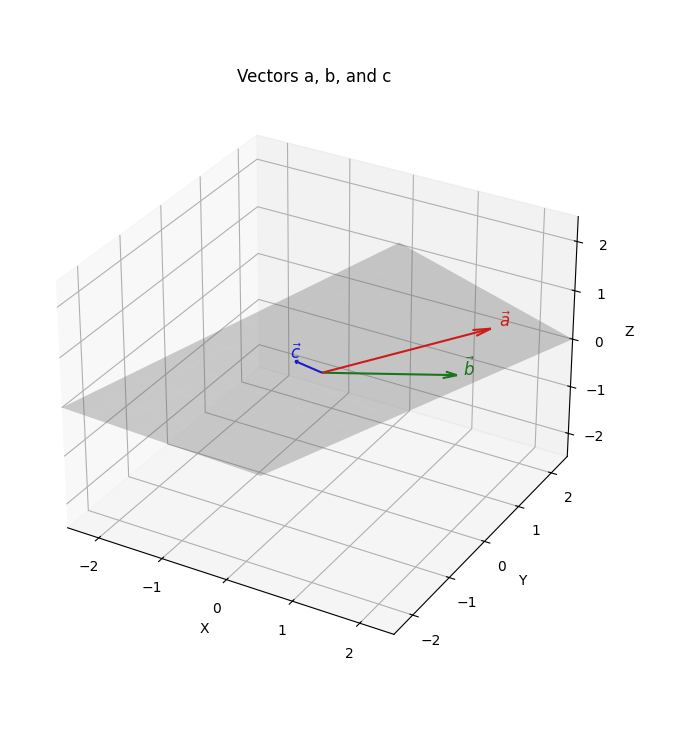
\includegraphics[height=0.6\textheight, keepaspectratio]{figs/q5.png}
\captionof{figure}{Graph}
\end{figure}
\end{document}